\usepackage{float}
\subsection{Pipeline Justification}\label{sec:pipeline-justification}

As introduced in the problem description, the router determines which of eight specialized agents should answer an incoming user query. Interhyp presented this component as part of its existing architecture, and improving its routing quality was the central goal of the project. This led to the requirement of developing an approach to first systematically evaluate routing quality. Without automation, this depends on manual work in two places. First, expected routing decisions need to be created manually. This requires building a golden dataset which contains the user query and the expected agent to which the query should be routed to. Second, understanding failure cases requires manual root cause analysis to identify common patterns among misrouted queries. Based on the results of the evaluation, the router's system prompt would have to be rewritten manually and validated through another round of manual assessment. As Interhyp's chatbot needs to handle more than 5,000 user queries per day, this does not scale at production volume.

The project title already points to the alternative. A Self-Improving Evaluation Pipeline should automatically improve itself without human intervention. This motivated a literature search for an automatic substitute of human routing assessment and prompt optimization. Using a large language model to evaluate the outputs of other models, referred to as LLM-as-a-Judge, is an established and actively researched paradigm \autocite{gu2024llmjudge}. The viability of this approach is also supported by \textcite{zheng2023judging}, who showed that well configured LLM judges can reach over 80\% agreement with human preferences, the same level of agreement as between humans. The concept was chosen as it fits Interhyp's use case well. An LLM judge can take over the two manual tasks identified above, assessing routing decisions and producing structured reasoning, that functions as an optimization signal to adjust the router prompt.

\begin{figure}[H]
\centering
\pandocbounded{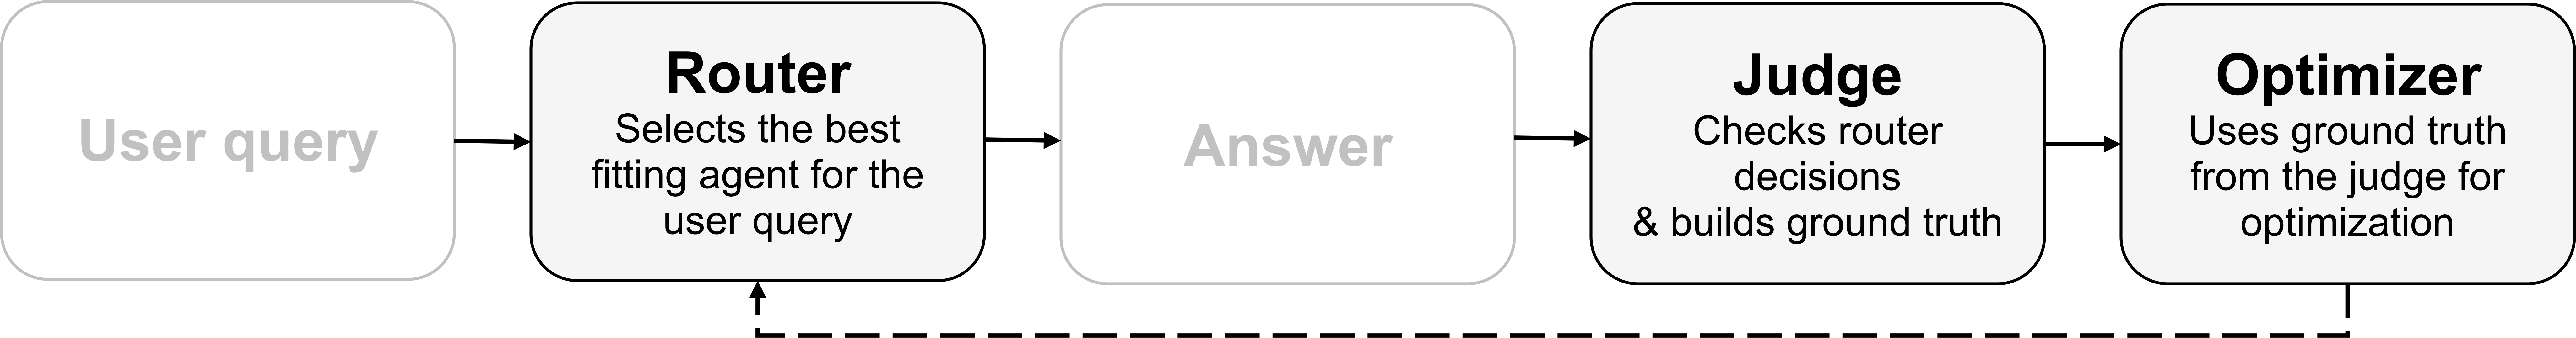
\includegraphics[keepaspectratio]{assets/pipeline/pipeline-architecture.png}}
\caption{High-level overview of the pipeline architecture (own illustration)}
\label{fig:pipeline-architecture}
\end{figure}


The resulting pipeline consists of three components with clearly separated responsibilities. The router makes the routing decision, the judge evaluates it, and the optimizer uses the judge's evaluations to improve the router's system prompt. Evaluation and improvement were deliberately split into two distinct modules rather than one component handling both. This aligns with the modularity principle used throughout the project (see \cref{sec:chatbot-application}) and reflects the design philosophy of \textcite{khattab2024dspy}, whose DSPy framework splits language model pipelines into small, specialized modules instead of components combining several tasks. The separation also keeps the judge's output reusable. The reasoning can later serve both as an evaluation record for humans and as the input signal for the optimizer. The following sections describe the three components in more detail.
